\documentclass{standalone}
\usepackage{pgfplots}
  \usepgflibrary{arrows.meta}

\usepackage{emerald}


\pgfplotsset{
  xkcd/.style={
    decoration={
      name=random steps,
      segment length=2pt,
      amplitude=0.3pt,
    },
    line width=1pt,
    line join=round,
    line cap=round,
    decorate,
  },
}
\pgfplotsset{
  xkcd axis/.style={%
    axis on top,
    xkcd,
    every non boxed x axis/.style={
      xtick align=center,
      enlarge x limits=true,
      x axis line style={-Straight Barb[round]}
    },
    every non boxed y axis/.style={
      ytick align=center,
      enlarge y limits=true,
      y axis line style={-Straight Barb[round]}
    },
    every tick/.append style={
      black,
      xkcd,
    },
    every axis plot post/.append style={
      double= . ,
      mark=none,
      draw=white,
      double distance=1pt,
    },
    every axis legend/.append style={
      xkcd,
    },
    tick label style={/pgf/number format/assume math mode=true},
    execute at begin axis={\ECFAugie},
  },
}


\begin{document}

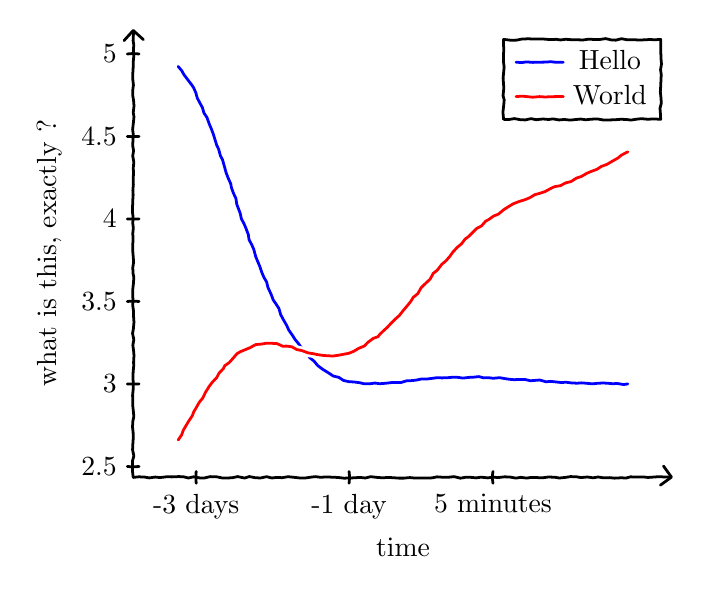
\begin{tikzpicture}
  \begin{axis}[%
    xkcd axis,
    axis x line=bottom,
    axis y line=left,
    xtick={1.2, 2.9, 4.5},
    xticklabels={-3 days, -1 day, 5 minutes},
    xlabel=time,
    ylabel={what is this, exactly ?},
    ]
    \addplot +[samples=30, domain=1:6] {3+(sin(deg(x))^2)/sqrt(x)*exp(-(x-2))};
    \addlegendentry{Hello}
    \addplot +[samples=30, domain=1:6] {0.4*x+2+x^2*sin(deg(x))^2*exp(-x)}; 
    \addlegendentry{World}
  \end{axis}
\end{tikzpicture}
\\{}\\
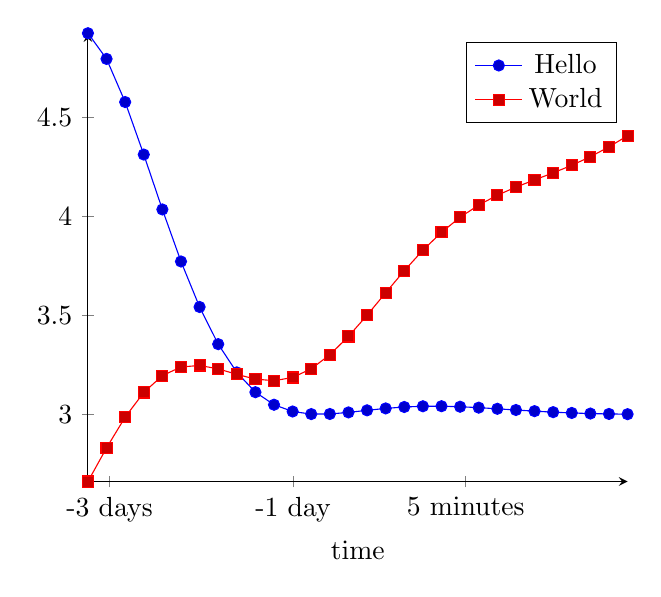
\begin{tikzpicture}
  \begin{axis}[%
    %xkcd axis,
    axis x line=bottom,
    axis y line=left,
    xtick={1.2, 2.9, 4.5},
    xticklabels={-3 days, -1 day, 5 minutes},
    xlabel=time,
    ]
    \addplot +[samples=30, domain=1:6] {3+(sin(deg(x))^2)/sqrt(x)*exp(-(x-2))};
    \addlegendentry{Hello}
    \addplot +[samples=30, domain=1:6] {0.4*x+2+x^2*sin(deg(x))^2*exp(-x)}; 
    \addlegendentry{World}
  \end{axis}
\end{tikzpicture}
\\
\end{document}